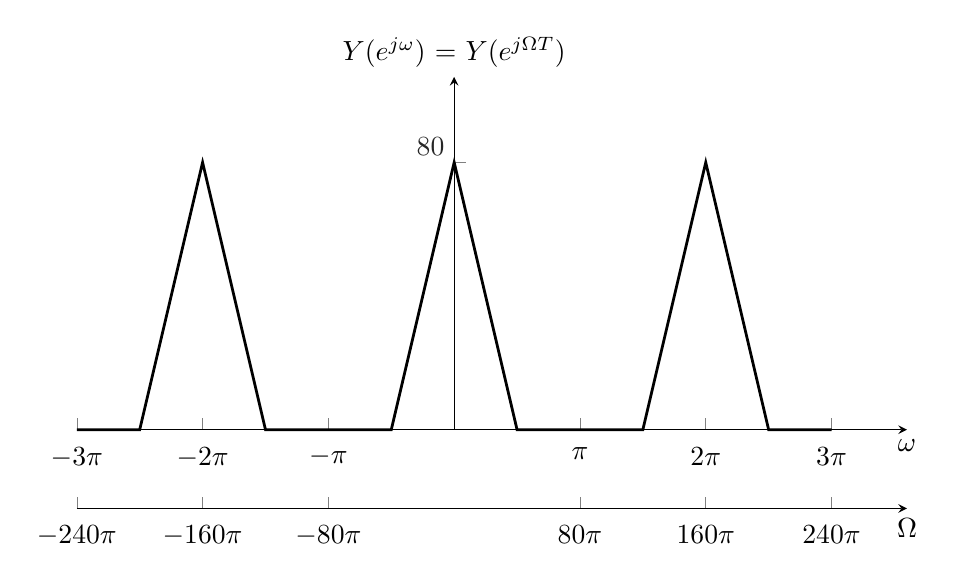
\begin{tikzpicture} 
\begin{axis}[
axis lines*=middle,
enlargelimits = upper, clip=false,
width=\textwidth,
height=0.5\textwidth,
ymin=0,
ymax=1.2,
xmin=-30,
xmax=30,
axis line style={->,>=stealth},
xlabel={$\omega$},
ylabel={$Y(e^{j\omega})$ = $Y(e^{j\Omega T})$},
yticklabel style = {yshift=0.2cm},
xticklabel style = {yshift=-0.1cm},
every axis x label/.style={
	at={(ticklabel* cs:1)},
	anchor=north,
},
every axis y label/.style={
	at={(ticklabel* cs:1)},
	anchor=south,
},
ytick=1,
yticklabels={$80$},
xtick={-30, -20, -10,  10, 20, 30},
xticklabels={$-3\pi$, $-2\pi$, $-\pi$, $\pi$, $2\pi$, $3\pi$},
every outer y axis line/.append style={white!15!black},
every y tick label/.append style={font=\color{white!15!black}},
legend style={draw=white!15!black,fill=white,legend cell align=left}]
%\addplot[black, line width=1.5pt] coordinates {(-30, 1) (30, 1)};
\addplot[black, line width=1pt, domain=-30:30, samples=101] coordinates {(-30, 0) (-25, 0) (-20, 1) (-15, 0) (-5, 0) (0, 1) (5, 0) (15, 0) (20, 1) (25, 0) (30, 0)};
\end{axis}

% extra x axis
\begin{axis}[yshift=-1cm,
axis lines*=middle,
enlargelimits = upper, clip=false,
xmin=-30,
xmax=30,
width=\textwidth,
height=0.5\textwidth,
hide y axis,
axis line style={->,>=stealth},
xlabel={$\Omega$},
xticklabel style = {yshift=-0.1cm},
every axis x label/.style={
	at={(ticklabel* cs:1)},
	anchor=north,
},
xtick={-30, -20, -10,  10, 20, 30},
xticklabels={$-240\pi$, $-160\pi$, $-80\pi$, $80\pi$, $160\pi$, $240\pi$},
every outer y axis line/.append style={white!15!black},
every y tick label/.append style={font=\color{white!15!black}},
legend style={draw=white!15!black,fill=white,legend cell align=left}]
\addplot[draw=none] {1};
\end{axis}

\end{tikzpicture}